\documentclass[11pt]{article}

%PRéAMBULE
\usepackage[utf8]{inputenc}
\usepackage[table,dvipsnames]{xcolor}
\usepackage[T1]{fontenc}
\usepackage[sort&compress,numbers]{natbib}
%\usepackage{multibib}
\usepackage[french]{babel}
\usepackage[normalem]{ulem}
\usepackage{verbatim}
\usepackage{graphicx}
\usepackage{graphics}
\usepackage{fancybox}
\usepackage{amsfonts}
\usepackage{amsmath}
\usepackage{ulem}
\usepackage{adjustbox}
\usepackage{amssymb,amsmath,latexsym}
\usepackage{mathrsfs}
\usepackage[a4paper]{geometry}
\usepackage{subfig}
\usepackage{placeins}
\usepackage{float}
\usepackage[bottom]{footmisc}
\usepackage{default}
\usepackage{multicol}
\usepackage{hyperref}


%TITRE
\geometry{hscale=0.8,vscale=0.8,centering}
\title{Théorie de l'information\\
	Suivi de projet\\
	Stéganographie dans les images}
\author{Gautier Darchen \\ Alexandre Huat \\ Romain Judic}
\date{\today}

\begin{document}
\maketitle
\noindent\rule{\textwidth}{1.3pt}

\section{Avancement du projet}

\subsection{Définition de la stéganographie}
La stéganographie permet de dissimuler un message (dit secondaire) dans un autre (dit primaire) tout en laissant le message primaire lisible de tous. Le message secondaire, lui, ne devra être lisible que par une personne possédant une information spéciale comme une clé ou une méthode d'extraction du message secondaire.\\

Il existe la stéganographie textuelle et la stéganographie dans les images. La stéganographie textuelle est très facile à déceler car elle n'offre pas vraiment d'autre choix que générer un texte incompréhensible, dont on comprend facilement qu'il cache quelque chose. La stéganographie dans les images est beaucoup plus efficace et il existe de très nombreuses méthodes pour cacher, extraire ou déceler un message dans une image\cite{VariousStego}.

\subsection{Exemples de méthodes de stéganographie}
Il existe plusieurs méthodes de stéganographie dans les images, nous en avons abordé trois :
\begin{itemize}
\item la stéganographie par substitution ;
\item la stéganographie par étalement de spectre ;
\item la stéganographie dans le domaine transformé.
\end{itemize}

\subsubsection{Stéganographie par substitution de LSB \emph{(LSB Replacement)}\cite{CoursUM2,Zath,PrincipMax}} % Got
%biblio : https://www.lirmm.fr/~wpuech/enseignement/master_informatique/Compression_Insertion/Dissimulation_de_donnees_Cours3.pdf
% https://histoiresecretes.wordpress.com/2013/05/05/la-steganographie-par-substitution/
% http://www.math.ucsd.edu/~crypto/Projects/MaxWeiss/steganography.pdf
\paragraph{Définition}~\\\indent
La stéganographie par substitution de \emph{LSB} (\emph{Least Significant Bit}) -- dans l'exemple de la stéganographie au travers d'une image -- consiste à substituer les bits de poids faibles (les \emph{LSB}) des pixels de l'image originale par les bits du message que l'on souhaite insérer. À la réception de l'image, le destinataire du message caché doit savoir au préalable dans quel sens parcourir les pixels pour retrouver le message (usuellement, parcours pseudo-aléatoire choisi, avec une clé secrète $k$).

\paragraph{Exemple}~\\\indent
\underline{Message ($M$) :} $M = 11001000$ ~\\\\\indent
\underline{Traitement de l'image en niveau de gris :} ~\\\indent
On découpe le message $M$=\textbf{\textcolor{red}{1}
						  \textcolor{blue}{1}
						  \textcolor{green}{0}
						  \textcolor{orange}{0}
						  \textcolor{gray}{1}
						  \textcolor{Brown}{0}
						  \textcolor{RubineRed}{0}
						  \textcolor{Violet}{0}}
 
 ~\\

\begin{minipage}{.5\textwidth}\centering
	\begin{tabular}{|c|c|c|c|}
	\hline
	00110100 & 11001010 & 01101001 & 11101101 \\\hline
	10000010 & 10100100 & 00101101 & 10111011 \\\hline
	\end{tabular}
	\captionof{table}{Image originale en niveaux de gris}
\end{minipage}
\begin{minipage}{.5\textwidth}\centering
	\begin{tabular}{|c|c|c|c|}
	\hline
	0011010\textcolor{red}{\textbf{1}} & 1100101\textcolor{blue}{\textbf{1}} & 0110100\textcolor{green}{\textbf{0}} & 1110110\textcolor{orange}{\textbf{0}} \\\hline
	1000001\textcolor{gray}{\textbf{1}} & 1010010\textcolor{Brown}{\textbf{0}} & 0010110\textcolor{RubineRed}{\textbf{0}} & 1011101\textcolor{Violet}{\textbf{0}} \\\hline
	\end{tabular}
	\captionof{table}{Image modifiée en niveaux de gris}
\end{minipage}

\paragraph{Application}~\\\indent
On utilise un programme \textsf{Matlab} permettant de réaliser de la stéganographie par substitution de \emph{LSB}. On fournit à ce programme deux images carrées de dimension similaires : l'une des images est la \emph{cover} (l'image dans laquelle on veut dissimuler un message), la seconde est l'image à cacher. Le programme transforme ensuite ces images en niveaux de gris. On choisit également le nombre de bits à substituer.\\

Voici un exemple d'application. La stéganographie est ici réalisée par substitution d'un seul bit : le bit de plus faible poids. 

\begin{minipage}{.5\textwidth}\centering
	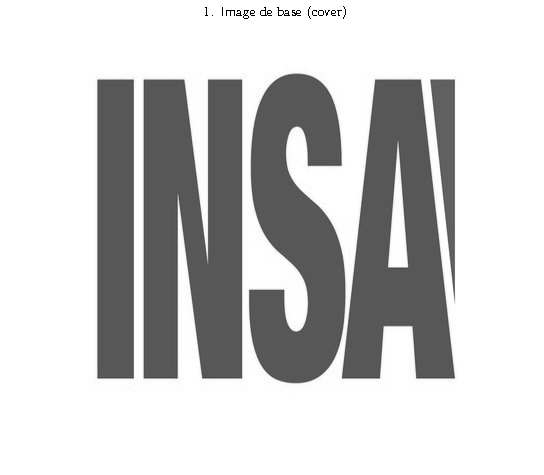
\includegraphics[scale=0.4]{images/fig1.png}
	\captionof{figure}{Image de base (\emph{cover})}
	\label{fig1}
\end{minipage}
\begin{minipage}{.5\textwidth}\centering
	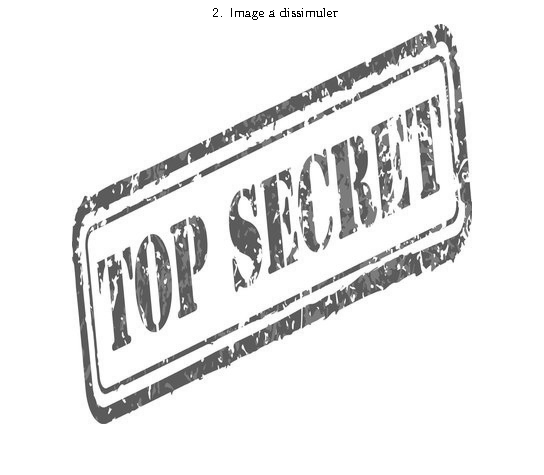
\includegraphics[scale=0.4]{images/fig2.png}
	\captionof{figure}{Image à dissimuler}
	\label{fig2}
\end{minipage}


\begin{minipage}{.5\textwidth}\centering
	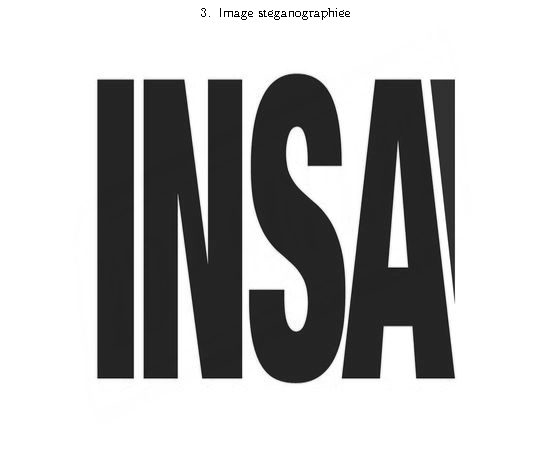
\includegraphics[scale=0.4]{images/fig3.png}
	\captionof{figure}{Image stéganographiée}
	\label{fig3}
\end{minipage}
\begin{minipage}{.5\textwidth}\centering
	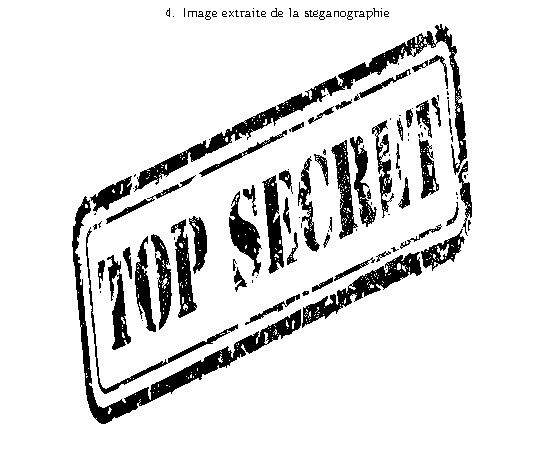
\includegraphics[scale=0.4]{images/fig4.png}
	\captionof{figure}{Image extraite de la stéganographie}
	\label{fig4}
\end{minipage}


\begin{minipage}{.5\textwidth}\centering
	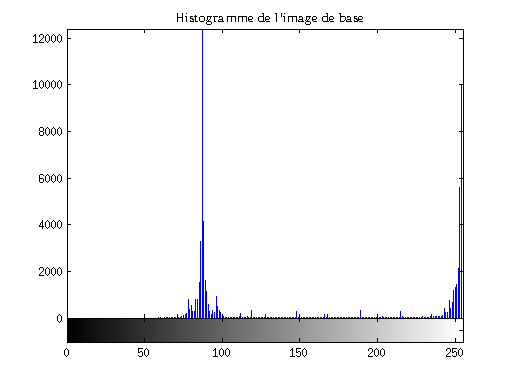
\includegraphics[scale=0.4]{images/fig5.png}
	\captionof{figure}{Histogramme de l'image \emph{cover}}
	\label{fig5}
\end{minipage}
\begin{minipage}{.5\textwidth}\centering
	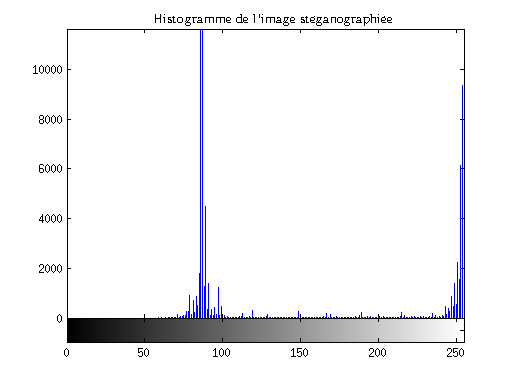
\includegraphics[scale=0.4]{images/fig6.png}
	\captionof{figure}{Histogramme de l'image stéganographiée}
	\label{fig6}
\end{minipage}

\paragraph{Commentaires}~\\\indent
Sur la figure \ref{fig3}, on ne voit pas à l'\oe il nu qu'un message est dissimulé. Pourtant, on voit bien sur la figure \ref{fig4} qu'un message caché a pu être extrait de l'image stéganographiée. Ce message caché est même récupéré sans trop de distorsion. Le programme nous renvoie les résultats suivants pour le PSNR\footnote{\emph{Peak Signal to Noise Ratio}.} et l'EQM\footnote{Erreur Quadratique Moyenne.} : 
$$ EQM = \frac{1}{m\cdot n}\sum_{i=0}^{m-1}\sum_{j=0}^{n-1}\big(I_1(i,j)-I_2(i,j) \big)^2 = 1.39\times 10^4$$
où $I_1$ représente l'image originale à dissimuler, $I_2$ est l'image dissimulée récupérée après la stéganographie, $m$ est la hauteur des images et $j$ est la largeur des images. L'EQM est relativement élevée puisqu'elle compare chaque pixel entre les deux images, et qu'ici les pixels sont modifiés, bien que très peu puisqu'on ne change que le bit de poids faible de certains des pixels, mais modifiés tout de même.
$$PSNR = 10\cdot \log_{10}\left(\frac{d^2}{EQM}\right) = 10.6027 $$
où $d$ est la dynamique du signal, donc ici la valeur maximale qu'un pixel peut avoir, soit $d=255$ dans notre cas (pixels codés sur 8 bits).

Enfin on voit sur les figures \ref{fig5} et \ref{fig6} que les histogrammes sont grossièrement identiques, ce qui est logique. En effet, seul le bit de plus faible poids est modifié ici. Ce bit est donc celui qui apporte le moins d'information sur chacun des pixels. Sa modification n'a donc pas un impact grave sur le pixel original.

\paragraph{Critique de cette méthode}
\begin{description}
\item[Avantage] Facile à implémenter et calculs de complexité relativement faible.
\item[Inconvénient] Assez facilement repérable et attaquable (attaque du $\chi^2$) car, bien que peu visible à l'\oe il nu, la distribution statistique du support est relativement altérée. 
\end{description}


\subsubsection{Stéganographie par étalement de spectre \emph{(SSIS : Spread Spectrum Image Steganography)}\cite{Patch,ARL-TR-1698}}
\paragraph{Définition}~\\\indent
La technique d'étalement de spectre consiste à dissimuler le message dans un bruit de même taille que l'image \emph{cover} et à l'additionner à cette dernière.
La modulation du message par le bruit permet d'étaler son spectre, c'est-à-dire de le rendre moins facile à détecter car ne présentant plus de motifs distincts.
On va utiliser un bruit de très faible puissance par rapport à celle de l'image. De cette manière, en additionnant ces deux derniers, l'image ne sera pas altérée visuellement.

\paragraph{Insertion}
\begin{itemize}
\item
On dispose du message $m$ et de la \emph{cover} $x$ de taille $n$
\item
On génère, grâce à une clé secrète, un bruit de taille $n$ et de faible puissance par rapport à celle de $x$ (la clé sera transmise au destinataire de l'image tatouée)
\item
On module le message $m$ par le bruit puis on l'étend spatialement (en le répliquant par exemple) $\rightarrow$ on obtient un signal $m_{b}$ de taille $n$
\item
On additionne pour obtenir $w$ le signal à envoyer : $w = x + m_{b}$
\end{itemize}

\paragraph{Extraction}~\\\indent
Pour récupérer le message $m$, le destinataire doit posséder la clé de génération du bruit. On doit disposer de techniques de restauration d'images pour continuer.
\begin{itemize}
\item
À partir de $w$, le décodeur produit une estimation $\hat{x}$ de l'image initiale
\item
$(w-\hat{x})$ correspond à la différence (estimée) entre l'image initiale et le signal reçu, c'est-à-dire à une estimation $\hat{m_{b}}$ du message bruité
\item
Grâce à la connaissance de la clé, on peut générer le bruit $b$ et donc démoduler une estimation du message $\hat{m}$
\end{itemize}

\paragraph{Exemple simple}~\\\indent
Pour illustrer la partie sur la modulation du message, soit $m$ un message bilatéral ($m_{i} \in \{-1,+1\}$) et $b$ un bruit gaussien $b$ généré grâce à une clé $k$ (par exemple $k = \sigma$).
~\\
\underline{Phase d'insertion :} on assigne simplement au bruit le signe du message à dissimuler.$$ w = m \times b $$
~\\
\underline{Phase d'extraction :} Après avoir identifié la partie correspondant au bruit sur l'image reçue, un simple examen des signes de $m_{b}$ permet de retrouver le message.$$ \hat{m} = signe(m_{b}) $$



\paragraph{Critique de cette méthode}
\begin{description}
\item[Avantages] Le tatouage est complètement invisible et difficilement décelable par analyse informatique.
\item[Inconvénients] L'extraction du message dissimulé nécessite la connaissance de techniques d'étalement spatial (pour donner au message la même taille que l'image) et de restauration d'image relativement complexes à mettre en \oe{}uvre.
\end{description}



% http://www.lia.deis.unibo.it/Courses/RetiDiCalcolatori/Progetti98/Fortini/patchwork.html
% http://www.dtic.mil/dtic/tr/fulltext/u2/a349102.pdf

%%% stego dans le domaine transformé
\subsubsection{Stéganographie dans le domaine transformé\cite{DWT-DCT,Ondelettes}}

\paragraph{Introduction}~\\\indent
Cette technique de stéganographie consiste à intégrer l'information secrète dans un domaine transformé du signal. Dans une image, on distingue le domaine spatial, basé sur les pixels, et son domaine transformé qui est celui des fréquences. Les techniques de stéganographie sur le domaine transformé utilisent la transformée orhtognale de l'image (exemple : transformée de Fourier discrète) plutôt que l'image elle-même. La transformée orthogonale ayant donc deux composantes, la magnitude et la phase.\\

Nous ne présentons ici qu'une des méthodes utilisées dans le domaine transformé : l'utilisation de la transformée d'ondelettes discrète (DWT, pour \emph{Discrete Wavelet Transform}).

\paragraph{Transformée d'ondelettes discrète (DWT)}~\\\indent
La DWT permet une décomposition hiérarchique d'une image. Elle se base sur l'utilisation d'ondelettes qui sont de fréquences et durées variables. Ces ondelettes permettent à la fois une description spatiale et fréquentielle de l'image : la DWT indique quelle fréquence apparaît, où, et sur quelle surface. La transformée en ondelettes détecte les zones riches en informations (à fort contraste) et les sépare. Une ondelette est une fonction de valeur moyenne nulle et limitée dans le temps. Les ondelettes sont générées par des translations, compressions et dilatations d'une ondelette mère. \\

L'application de la DWT, consiste à filtrer l'image dans les deux dimensions (filtrage vertical, horizontal et diagonal). Ces filtres décomposent l'image en 4 parties (sous-bandes) de résolution inférieure. Ces sous-bande sont sans chevauchement et ont différentes résolutions, on les nomme LL, LH, HL et HH. La sous-bande LL correspond aux coefficients de corrélation déterminés par une fonction d'ondelette dilatée jouant le même rôle qu'un filtre passe bas. Les autres sous bandes montrent les valeurs déterminées par la fonction d'ondelette mère compressée, faisant office de filtres passe haut. On peut appliquer plusieurs DWT à la suite, on le fait alors sur la sous-bande LL. Après $N$ DWT on se retrouve ainsi avec $3N+1$ sous-bandes.\\

Par sa capacité à bien représenter les fréquences dans l'espace, la DWT est très efficace pour la stéganographie. En effet, la plus grande quantité d'énergie dans l'image est stockée dans les basses fréquences (sous-bande LL$_{N}$). Ainsi, cacher un message en basse fréquence altérerait beaucoup la qualité de l'image et serait facilement décelable, même si cela serait plus robuste. Par conséquent, cacher un message dans les hautes fréquences (sous-bandes LH$_{X}$ et HL$_{X}$) serait bien plus discret car l'\oe il humain remarque difficilement les changements dans les contours.\\

\begin{figure}[h]
\centering
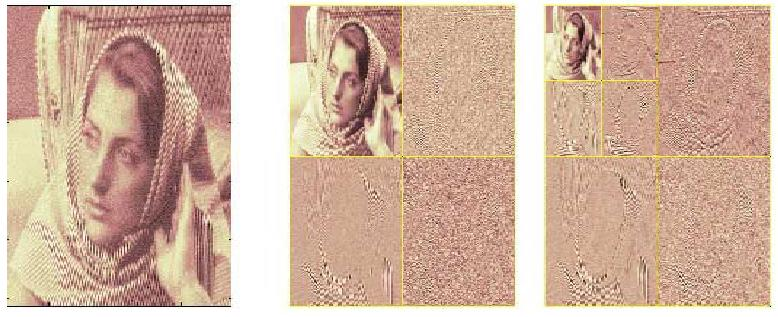
\includegraphics[width=\linewidth]{images/dwt-exemple.jpg}
\caption{Exemple de deux DWT successives (sur l'image du milieu : LL en haut à gauche, LH en bas à gauche, HL en haut à droite, HH en bas à droite)}
\end{figure}

\paragraph{Algorithme générique d'implantation et d'extraction d'un message}~\\\indent
\subparagraph{Implantation d'un message secret}
\begin{enumerate}
\item Étudier l'image et le message secret (texte/image) pour trouver la meilleure manière de le cacher.
\item Transformer le message en fichier binaire s'il ne l'est pas encore. Réaliser une DWT sur l'image de couverture.
\item Déterminer les coefficients de filtrage dans les directions verticale et horizontale (LH et HL). Cacher les bits du message dans ces coefficients (remplacement).
\item Créer la stego-image (par transformée inverse IDWT).
\end{enumerate}

\subparagraph{Extraction d'un message secret}
\begin{enumerate}
\item Étudier la stego-image pour savoir comment a pu être dissimulé le message.
\item Calculer la DWT et extraire les coefficients de filtrage verticaux et horizontaux.
\item Reconstruire le message bits par bits à partir des coefficients.
\item Recomposer le message compréhensible par l'humain.
\end{enumerate}

\begin{figure}[h]
	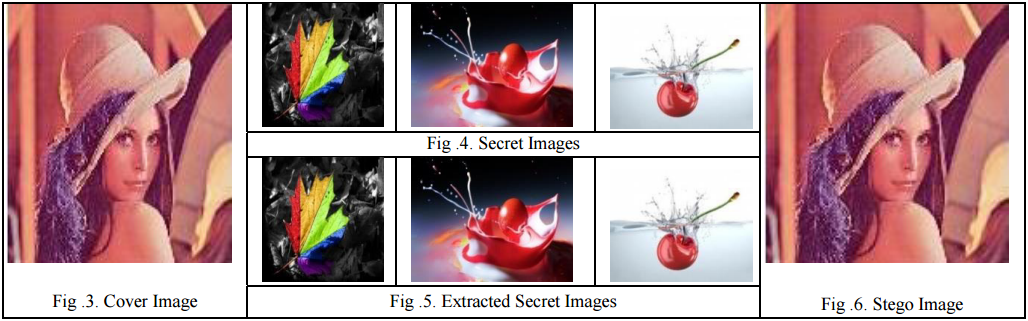
\includegraphics[width=\linewidth]{images/dwt-stego-exemple.png}
	\centering \caption{Exemple de stéganographie avec une DWT : implantation de trois images secrètes dans une seule en utilisant les trois canaux RGB\cite{DWT-RGB}}
\end{figure}

\paragraph{Commentaire}~\\\indent
La DWT est une des transformations les plus robustes et les plus efficaces pour la stéganographie dans le domaine transformé. Elle ne permet pas de cacher un gros volume de données mais assure une forte invisibilité du message, une forte robustesse contre les traitements d'image ultérieurs et permet une faible détérioration du message à l'extraction. Elle est souvent présentée comme la méthode la plus sûre pour la stéganographie dans le domaine transformé.

\section{Répartition des tâches}
\begin{description}
\item[Gautier :] stéganographie par substitution de LSB (voir code Matlab).
\item[Romain :] stéganographie par étalement de spectre (SSIS).
\item[Alexandre :] stéganographie dans le domaine transformé.
\end{description}

\section{Suite envisagée du projet}
\begin{itemize}
	\item S'intéresser aux techniques de détection de message stéganographiés et de comparaison de méthodes de stéganographie.
	\item Coder des exemples de stéganographie.
\end{itemize}

\bibliography{biblio}
\bibliographystyle{ieeetr}

\end{document}